\documentclass{article}
\usepackage[utf8x]{inputenc}
\usepackage{ucs}
\usepackage{amsmath} 
\usepackage{amsfonts}
\usepackage{marvosym}
\usepackage{wasysym}
\usepackage{upgreek}
\usepackage[english,russian]{babel}
\usepackage{graphicx}
\usepackage{float}
\usepackage{textcomp}
\usepackage{hyperref}
\usepackage{geometry}
  \geometry{left=2cm}
  \geometry{right=1.5cm}
  \geometry{top=1cm}
  \geometry{bottom=2cm}
\usepackage{tikz}
\usepackage{ccaption}
\usepackage{multicol}

\hypersetup{
   colorlinks=true,
   citecolor=blue,
   linkcolor=black,
   urlcolor=blue
}

\usepackage{listings}
%\setlength{\columnsep}{1.5cm}
%\setlength{\columnseprule}{0.2pt}

\usepackage[absolute]{textpos}

\usepackage{colortbl,graphicx,tikz}
\definecolor{X}{rgb}{.5,.5,.5}


\begin{document}
\pagenumbering{gobble}
\lstset{
  language=C,                % choose the language of the code
  basicstyle=\linespread{1.1}\ttfamily,
  columns=fixed,
  fontadjust=true,
  basewidth=0.5em,
  keywordstyle=\color{blue}\bfseries,
  commentstyle=\color{gray},
  stringstyle=\ttfamily\color{orange!50!black},
  showstringspaces=false,
  numbersep=5pt,
  numberstyle=\tiny\color{black},
  numberfirstline=true,
  stepnumber=1,                   % the step between two line-numbers.        
  numbersep=10pt,                  % how far the line-numbers are from the code
  backgroundcolor=\color{white},  % choose the background color. You must add \usepackage{color}
  showstringspaces=false,         % underline spaces within strings
  captionpos=b,                   % sets the caption-position to bottom
  breaklines=true,                % sets automatic line breaking
  breakatwhitespace=true,         % sets if automatic breaks should only happen at whitespace
  xleftmargin=.2in,
  extendedchars=\true,
  keepspaces = true,
}
\lstset{literate=%
   *{0}{{{\color{red!20!violet}0}}}1
    {1}{{{\color{red!20!violet}1}}}1
    {2}{{{\color{red!20!violet}2}}}1
    {3}{{{\color{red!20!violet}3}}}1
    {4}{{{\color{red!20!violet}4}}}1
    {5}{{{\color{red!20!violet}5}}}1
    {6}{{{\color{red!20!violet}6}}}1
    {7}{{{\color{red!20!violet}7}}}1
    {8}{{{\color{red!20!violet}8}}}1
    {9}{{{\color{red!20!violet}9}}}1
}
\newpage

\title{Семинар \#9: Память. Домашнее задание.\vspace{-5ex}}\date{}\maketitle

\section*{Задача 1: Создание указателей}
Решения всех подзадач этой части -- одна строка. Результат выполнения задания -- \texttt{.txt} файл, который содержит все эти строки.
\begin{enumerate}
\item В следующей программе создаётся переменная \texttt{a} типа \texttt{int}:
\begin{lstlisting}
int main() 
{
    int a = 1234;
    // Тут нужно написать 1 строку кода
}
\end{lstlisting}
Создайте указатель \texttt{p} и инициализируйте его адресом переменной \texttt{a}.


\item В следующей программе создаётся переменная \texttt{a} типа \texttt{double}:
\begin{lstlisting}
int main() 
{
    double a = 12.34;
    // Тут нужно написать 1 строку кода
}
\end{lstlisting}
Создайте указатель \texttt{p} и инициализируйте его адресом переменной \texttt{a}.

\item В следующей программе создаётся переменная \texttt{a} типа \texttt{char}:
\begin{lstlisting}
int main() 
{
    char a = ')';
    // Тут нужно написать 1 строку кода
}
\end{lstlisting}
Создайте указатель \texttt{p} и инициализируйте его адресом переменной \texttt{a}.

\item В следующей программе создаётся массив \texttt{array} из элементов типа \texttt{int}:
\begin{lstlisting}
int main() 
{
    int array[5] = {10, 20, 30, 40, 50};
    // Тут нужно написать 1 строку кода
}
\end{lstlisting}
Создайте указатель \texttt{p} и сделайте так, чтобы он указывал на первый элемент массива (индекс \texttt{0}).


\item В следующей программе создаётся строка -- массив \texttt{str} из элементов типа \texttt{char}:
\begin{lstlisting}
int main() 
{
    char str[20] = "Sapere Aude";
    // Тут нужно написать 1 строку кода
}
\end{lstlisting}
Создайте указатель \texttt{p} и сделайте так, чтобы он указывал на символ \texttt{'A'}  из строки \texttt{str}.

\newpage
\item В следующей программе создаётся структура \texttt{Book} из семинара про структуры:
\begin{lstlisting}
struct book 
{
    char title[50];
    int pages;
    float price;
};
typedef struct book Book;

int main() 
{
    Book b = {"Fahrenheit 451", 400, 700.0};

}
\end{lstlisting}

\begin{enumerate}
\item Создайте указатель \texttt{pb} и сделайте так, чтобы он указывал на структуру \texttt{b}.
\item Создайте указатель \texttt{pprice} и сделайте так, чтобы он указывал на поле \texttt{price} структуры \texttt{b}.
\item Создайте указатель \texttt{pc} и сделайте так, чтобы он указывал символ \texttt{'t'} поля \texttt{title} структуры \texttt{b}.
\end{enumerate} 


\item В следующей программе создаётся переменная \texttt{a} типа \texttt{float} и \texttt{p} указатель, который хранит её адрес:
\begin{lstlisting}
int main() 
{
    float a = 1.2;
    float* p = &a;
    // Тут нужно написать 1 строку кода
}
\end{lstlisting}
Создайте указатель \texttt{pp} и сделайте так, чтобы он указывал на указатель \texttt{p}.


\item В следующей программе создаётся структура \texttt{Book} из семинара про структуры и указатель на неё:
\begin{lstlisting}
struct book 
{
    char title[50];
    int pages;
    float price;
};
typedef struct book Book;

int main() 
{
    Book b = {"Fahrenheit 451", 400, 700.0};
    Book pb = &b;
    // Тут нужно написать 1 строку кода
}
\end{lstlisting}
Создайте указатель \texttt{ppb} и сделайте так, чтобы он указывал на указатель \texttt{pb}.


\end{enumerate}

\newpage
\section*{Задача 2: Использование указателей}
Решения всех подзадач этой части -- одна строка. Результат выполнения задания -- \texttt{.txt} файл, который содержит все эти строки.
\begin{enumerate}
\item В следующей программе была создана переменная \texttt{a} и указатель на неё \texttt{p}. Удвойте значение переменной \texttt{a}, используя только указатель \texttt{p}. Нужно использовать указатель \texttt{p}, саму переменную \texttt{a} использовать нельзя.
\begin{multicols}{2}
\begin{lstlisting}
#include <stdio.h>
int main() 
{
    int a = 1234;
    int* p = &a;
    // Тут нужно написать 1 строку кода
    
    printf("%i\n", a);
}
\end{lstlisting}

\vfill \null    
\columnbreak
\vfill \null 

\begin{center}
\vspace{1cm} 
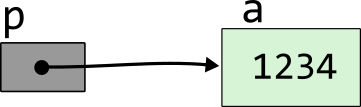
\includegraphics[scale=1]{../images/pointer_schemes/pointer_to_int.png}
\end{center}
\end{multicols}

\item В следующей программе была создана переменная \texttt{a} типа \texttt{float} и указатель на неё \texttt{p}. Возведите значение переменной \texttt{a} в квадрат, используя только указатель \texttt{p}. Нужно использовать только указатель \texttt{p}, саму переменную \texttt{a} использовать нельзя.
\begin{multicols}{2}
\begin{lstlisting}
#include <stdio.h>
int main() 
{
    float a = 1.5;
    float* p = &a;
    // Тут нужно написать 1 строку кода
    
    printf("%f\n", a);
}
\end{lstlisting}

\vfill \null    
\columnbreak
\vfill \null 

\begin{center}
\vspace{1cm} 
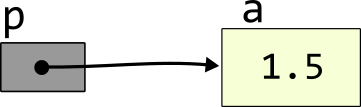
\includegraphics[scale=1]{../images/pointer_schemes/pointer_to_float.png}
\end{center}
\end{multicols}


\item В следующей программе была создана переменная \texttt{a} типа \texttt{char} и указатель на неё \texttt{p}. Переведите символ, хранящийся в переменной \texttt{a} в верхний регистр, используя только указатель \texttt{p}. Нужно использовать только указатель \texttt{p}, саму переменную \texttt{a} использовать нельзя.
\begin{multicols}{2}
\begin{lstlisting}
#include <stdio.h>
int main() 
{
    char a = 't';
    char* p = &a;
    // Тут нужно написать 1 строку кода
    
    printf("%c\n", a);
}
\end{lstlisting}

\vfill \null    
\columnbreak
\vfill \null 

\begin{center}
\vspace{1cm} 
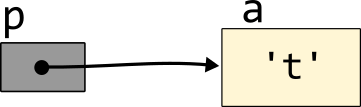
\includegraphics[scale=1]{../images/pointer_schemes/pointer_to_char.png}
\end{center}
\end{multicols}


\newpage
\item В следующей программе был создан массив \texttt{array} переменных  типа \texttt{int} и указатель \texttt{p} на первый элемент массива. 
\begin{multicols}{2}
\begin{lstlisting}
#include <stdio.h>
int main() 
{
    int array[5] = {10, 20, 30, 40, 50};
    int* p = &array[0];

    for (int i = 0; i < 5; ++i) 
        printf("%i ", array[i]);
}
\end{lstlisting}
\vfill \null    
\columnbreak
\vfill \null 
\begin{center}
\vspace{1cm} 
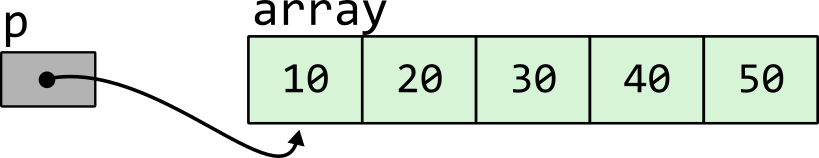
\includegraphics[scale=0.8]{../images/pointer_schemes/pointer_to_int_array.png}
\end{center}
\end{multicols}

\begin{enumerate}
\item Добавьте \texttt{1} к первому элементу массива (\texttt{array[0]}), используя только указатель \texttt{p}. Нужно использовать только указатель \texttt{p}, сам массив \texttt{array} использовать нельзя. Решение -- 1 строка.
\item Добавьте \texttt{1} к четвёртому элементу массива (\texttt{array[3]}), используя только указатель \texttt{p}. Нужно использовать только указатель \texttt{p}, сам массив \texttt{array} использовать нельзя. Менять \texttt{p} тоже нельзя. Решение -- 1 строка.

\item Добавьте \texttt{1} ко всем элементам массива. Нужно использовать только указатель \texttt{p}, сам массив \texttt{array} использовать нельзя. Решение -- 1 цикл.
\end{enumerate}


\item В следующей программе был создан массив \texttt{array} переменных  типа \texttt{int} и указатель \texttt{p} на четвёртый элемент массива (\texttt{array[3]}). 
\begin{multicols}{2}
\begin{lstlisting}
#include <stdio.h>
int main() 
{
    int array[5] = {10, 20, 30, 40, 50};
    int* p = &array[3];
    
    for (int i = 0; i < 5; ++i)
        printf("%i ", array[i]);
}
\end{lstlisting}
\vfill \null    
\columnbreak
\vfill \null 
\begin{center}
\vspace{1cm} 
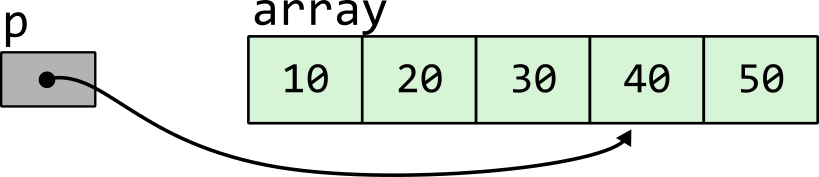
\includegraphics[scale=0.8]{../images/pointer_schemes/pointer_to_int_array_index4.png}
\end{center}
\end{multicols}

\begin{enumerate}
\item Добавьте \texttt{1} к первому элементу массива (\texttt{array[0]}), используя только указатель \texttt{p}. Нужно использовать только указатель \texttt{p}, сам массив \texttt{array} использовать нельзя. Менять \texttt{p} тоже нельзя. Решение -- 1 строка.
\item Добавьте \texttt{1} к пятому элементу массива (\texttt{array[4]}), используя только указатель \texttt{p}. Нужно использовать только указатель \texttt{p}, сам массив \texttt{array} использовать нельзя. Менять \texttt{p} тоже нельзя. Решение -- 1 строка.
\item Добавьте \texttt{1} ко всем элементам массива. Нужно использовать только указатель \texttt{p}, сам массив \texttt{array} использовать нельзя. Решение -- 1 цикл.
\end{enumerate}



\newpage
\item В следующей программе была создана строка \texttt{str} и указатель \texttt{p} на первый символ строки. 
\begin{multicols}{2}
\begin{lstlisting}
#include <stdio.h>
int main() 
{
    int str[] = "sapere aude";
    int* p = &str[0];

    printf("%s\n", str);
}
\end{lstlisting}
\vfill \null    
\columnbreak
\vfill \null 
\begin{center}
\vspace{1cm} 
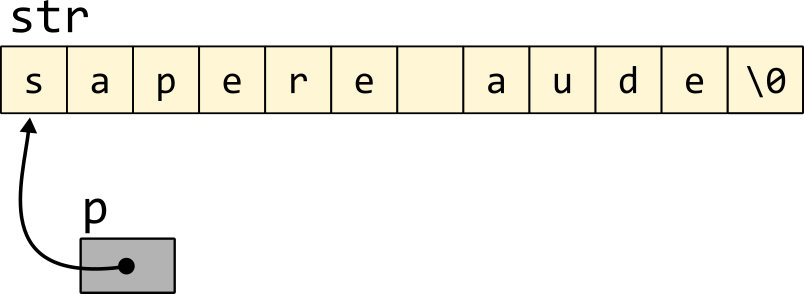
\includegraphics[scale=0.8]{../images/pointer_schemes/pointer_to_char_array.png}
\end{center}
\end{multicols}

\begin{enumerate}
\item Переведите в верхний регистр первую букву строки, используя только указатель \texttt{p}. Нужно использовать только указатель \texttt{p}, саму строку \texttt{str} использовать нельзя. Решение -- 1 строка.
\item Переведите в верхний регистр первую букву второго слова строки, используя только указатель \texttt{p}. Нужно использовать только указатель \texttt{p}, саму строку \texttt{str} использовать нельзя. Решение -- 1 строка.

\item Переведите в верхний регистр все буквы строки, используя только указатель \texttt{p}. Нужно использовать только указатель \texttt{p}, саму строку \texttt{str} использовать нельзя. Решение -- 1 цикл
\end{enumerate}


\item В следующей программе есть переменная \texttt{a} типа \texttt{int}, указатель \texttt{p} на эту переменную и указатель \texttt{q} на \texttt{p}. Удвойте значение переменной \texttt{a}, используя только указатель \texttt{q}. Нужно использовать только указатель \texttt{q}.
\begin{multicols}{2}
\begin{lstlisting}
#include <stdio.h>
int main() 
{
    int a = 1234;
    int* p = &a;
    int** q = &p;
    // Тут нужно написать 1 строку кода
    printf("%i\n", a);
}
\end{lstlisting}

\vfill \null    
\columnbreak
\vfill \null 


\begin{center}
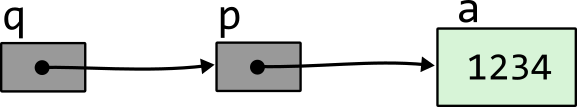
\includegraphics[scale=1]{../images/pointer_schemes/pointer_to_pointer_to_int.png}
\end{center}
\end{multicols}
\item В следующей программе была создана структура \texttt{a} типа \texttt{Date} и указатель на эту структуру. Добавьте \texttt{1} к значению поля \texttt{year}, используя только указатель \texttt{p}.
\begin{multicols}{2}
\begin{lstlisting}
#include <stdio.h>
struct date 
{
    int day, month, year;
};
typedef struct date Date;
int main() 
{
    Date a = {15, 5, 1970};
    Date* p = &a;
    // Тут нужно написать 1 строку кода
    printf("%d %d %d\n", 
           a.day, a.month, a.year);
}
\end{lstlisting}

\vfill \null    
\columnbreak
\vfill \null 

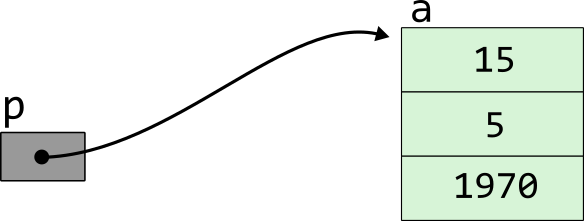
\includegraphics[scale=1]{../images/pointer_schemes/pointer_to_struct_date.png}
\end{multicols}

\newpage


\item В следующей программе была создана структура \texttt{a} типа \texttt{Movie} и указатель на неё.
\begin{multicols}{2}
\begin{lstlisting}
#include <stdio.h>
struct date 
{
    int day, month, year;
};
typedef struct date Date;

struct movie 
{
    char title[50];
    float rating;
    Date release_date;
};
typedef struct movie Movie;
\end{lstlisting}

\vfill \null  
\columnbreak
\vfill \null  

\begin{center}
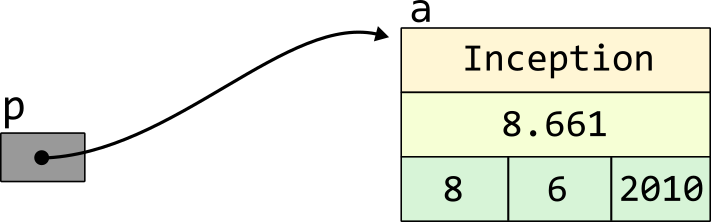
\includegraphics[scale=1]{../images/pointer_schemes/pointer_to_struct_movie.png}
\end{center}
\end{multicols}

\vspace{-10ex}
\begin{lstlisting}
int main() 
{
    Movie a = {"Inception", 8.661, {8, 6, 2010}};
    Movie* p = &a;
    // Тут нужно написать 1 строку кода
}
\end{lstlisting}
\begin{enumerate}
\item Увеличьте на \texttt{1} значение поля \texttt{rating}, используя только указатель \texttt{p}.
\item Увеличьте на \texttt{1} значение поля месяца выхода фильма, используя только указатель \texttt{p}.
\end{enumerate}





\item В следующей программе был создан массив \texttt{array} из структур типа \texttt{Movie} и указатель \texttt{p}, который указывает на второй элемент массива (\texttt{array[1]}).
\begin{lstlisting}
#include <stdio.h>
struct date 
{
    int day, month, year;
};
typedef struct date Date;

struct movie 
{
    char title[50];
    float rating;
    struct date release_date;
};
typedef struct movie Movie;

int main() 
{
    Movie array[3] = {{"Inception", 8.661, {8, 6, 2010}}, 
                      {"Green Mile", 9.062, {6, 12, 1999}}, 
                      {"Leon", 8.679, {14, 9, 1994}}};
    Movie* p = &array[1];
}
\end{lstlisting}

\vspace{-59ex}
\begin{center}
\quad\quad\quad\quad\quad\quad\quad\quad\quad\quad\quad\quad\quad\quad\quad\quad\quad\quad\quad\quad\quad\quad\quad
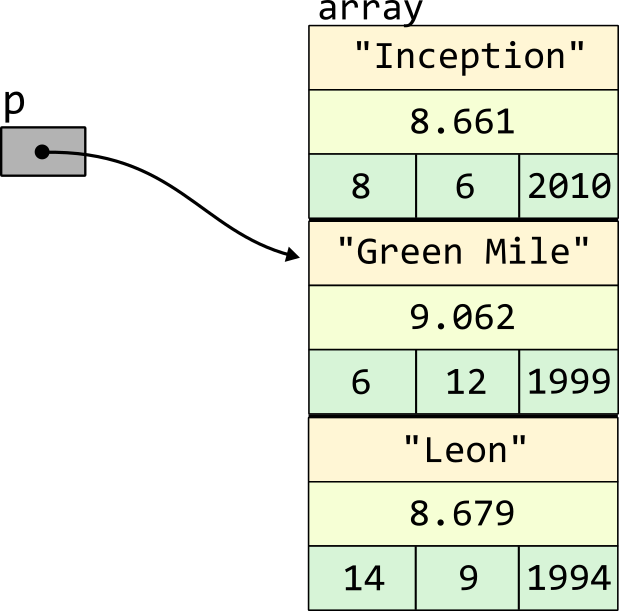
\includegraphics[scale=1]{../images/pointer_schemes/pointer_to_array_of_struct_movie.png}
\end{center}

\begin{enumerate}
\item Увеличьте на \texttt{1} значение рейтинга фильма \texttt{Inception}, используя только указатель \texttt{p}. При этом менять \texttt{p} нельзя, он  должен указывать на \texttt{array[1]}.
\item Удвойте значение года выхода фильма \texttt{Leon}, используя только указатель \texttt{p}. При этом менять \texttt{p} нельзя, он  должен указывать на \texttt{array[1]}.
\end{enumerate}

\end{enumerate}

\newpage
\section*{Задача 3: Передача в функцию по указателю}
\subsection*{Передача в функцию по значению}
\begin{multicols}{2}
\begin{lstlisting}
#include <stdio.h>

struct movie 
{
    char title[50];
    float rating;
    struct date release_date;
};
typedef struct movie Movie;

void change_rating(Movie m) 
{
    m.rating += 1;
}
int main() 
{
    Movie a = {"Inception", 8.661, 
                {8, 6, 2010}};
    change_rating(a);
}
\end{lstlisting}
\columnbreak
\begin{center}
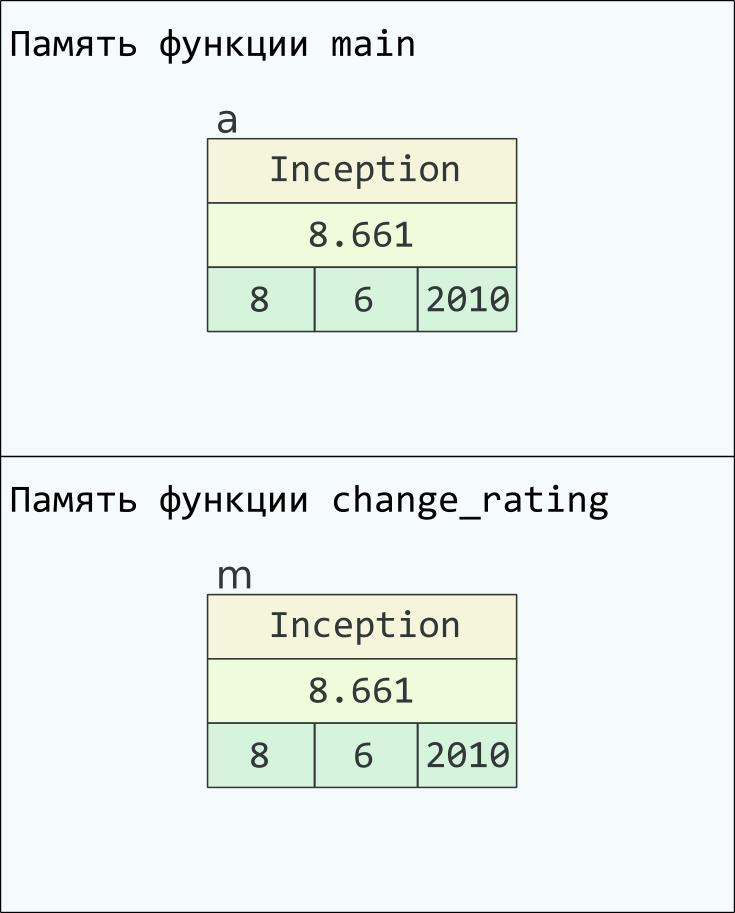
\includegraphics[scale=0.86]{../images/pointer_schemes/function_by_value.png}
\end{center}
\end{multicols}
Всё, что передаётся в функцию, копируется. Поэтому функция \texttt{change\_rating} будет менять
поле \texttt{rating} у копии структуры \texttt{a}, а изначальная структура не изменится.

\subsection*{Передача в функцию по указателю:}
\begin{multicols}{2}
\begin{lstlisting}
#include <stdio.h>
struct movie 
{
    char title[50];
    float rating;
    struct date release_date;
};
typedef struct movie Movie;

void change_rating(Movie* pm) 
{
    pm->rating += 1;
}
int main() 
{
    Movie a = {"Inception", 8.661, 
              {8, 6, 2010}};
    Movie* p = &a;
    change_rating(&a);
}
\end{lstlisting}
\columnbreak
\begin{center}
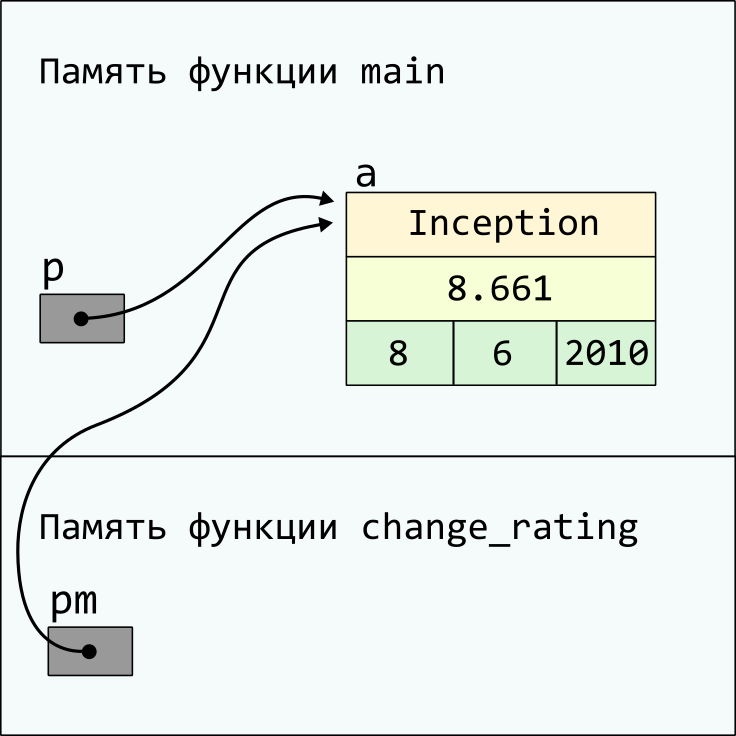
\includegraphics[scale=0.86]{../images/pointer_schemes/function_by_pointer.png}
\end{center}
\end{multicols}
Всё, что передаётся в функцию, копируется. Но теперь туда копируется указатель, который содержит
адрес стурктуры \texttt{a}. Используя этот указатель, мы можем изменить изначальную структуру. Более того, так как указатель занимает меньше памяти, его копирования в функцию происходит быстрее, чем копирование всей структуры.

\subsection*{Подзадачи:}
\begin{enumerate}
\item Напишите функцию \texttt{void inc(int* p)}, которая будет принимать на вход указатель на переменную типа \texttt{int} и увеличивать на \texttt{1} эту переменную. Протестируйте функцию, вызвав её из функции \texttt{main} с помощью следующего кода:
\begin{lstlisting}
#include <stdio.h>
// Тут вам нужно написать функцию inc

int main() 
{
    int a = 20;
    inc(&a);
    printf("%i\n", a); // Должно напечатать 21
}
\end{lstlisting}
\item Напишите функцию \texttt{void cube(float* p)}, которая будет принимать на вход указатель на переменную типа \texttt{float} и возводиить в куб эту переменную. Протестируйте функцию, вызвав её из функции \texttt{main} с помощью следующего кода: 
\begin{lstlisting}
#include <stdio.h>
// Тут вам нужно написать функцию cube

int main() 
{
    float a = 1.5;
    cube(&a);
    printf("%f\n", a); // Должно напечатать 3.375
}
\end{lstlisting}

\item Напишите функцию \texttt{void to\_upper(char* p)}, которая будет принимать на вход указатель на переменную типа \texttt{char} и, если символ, на который указывает этот указатель, является строчной буквой, функция должна делать эту букву заглавной. Протестируйте функцию, вызвав её из функции \texttt{main} с помощью следующего кода: 
\begin{lstlisting}
#include <stdio.h>
// Тут вам нужно написать функцию to_upper

int main() 
{
    char a = 't';
    to_upper(&a);
    printf("%c\n", a); // Должно напечатать T
}
\end{lstlisting}

\newpage
\item Напишите функцию \texttt{void inc\_array(int* p, int size)}, которая будет принимать на вход указатель на первый элемент массива и целое число \texttt{size} -- размер массива. Функция должна увеличивать на \texttt{1} все элементы массива. Протестируйте функцию, вызвав её из функции \texttt{main} с помощью следующего кода:
\begin{lstlisting}
#include <stdio.h>
// Тут вам нужно написать функцию inc_array

int main() 
{
    int a[5] = {10, 20, 30, 40, 50};
    inc_array(a, 5); 
    
    for (int i = 0; i < 5; ++i)
        printf("%i ", a[i]); 
    // Цикл должен напечатать 11 21 31 41 51
}
\end{lstlisting}
\item Напишите функцию \texttt{void string\_to\_upper(char* p)}, которая будет принимать на вход указатель на первый символ строки и переводить эту строку в верхний регистр.

\item Напишите функцию \texttt{void trim\_after\_first\_space(char* p)}, которая будет принимать на вход указатель на первый символ строки и укорачивать строку до первого пробела. Протестируйте функции, вызвав её их из функции \texttt{main} с помощью следующего кода:
\begin{lstlisting}
#include <stdio.h>
// Тут вам нужно написать функции string_to_upper и trim_after_first_space
int main() 
{
    char a[] = "Sapere Aude";
    string_to_upper(a);
    printf("%s\n", a); // Должно напечатать SAPERE AUDE
    trim_after_first_space(a);
    printf("%s\n", a); // Должно напечатать SAPERE
}
\end{lstlisting}

\item Напишите функцию \texttt{void increase\_rating(Movie* p)}, которая будет принимать указатель типа \texttt{Movie*} и увеличивать рейтинг фильма, на которой указывает \texttt{p}, на 1.

\newpage
\item Напишите функцию \texttt{void change\_year\_of\_movies(Movie* p, int size)}, которая принимает на вход указатель на первый элемент массива структур типа \texttt{Movie} и размер этого массива. Функция должна увеличивать год выхода всех фильмов на \texttt{1}. Протестируйте функции, вызвав их из функции \texttt{main} с помощью следующего кода:

\begin{lstlisting}
#include <stdio.h>
struct date 
{
    int day, month, year;
};
typedef struct date Date;
struct movie 
{
    char title[50];
    float rating;
    struct date release_date;
};
typedef struct movie Movie;

void print_date(const Date* pd) 
{
    printf("%02d.%02d.%04d", pd->day, pd->month, pd->year);
}
void print_movie(const Movie* pm) 
{
    printf("Title: %s\nRating: %.2f\nDate: ", pm->title, pm->rating);
    print_date(&pm->release_date);
    printf("\n");
}
// Тут вам нужно написать функции increase_rating и change_year_of_movies

int main() 
{
    Movie a[3] = {{"Inception", 8.661, {8, 6, 2010}}, 
                  {"Green Mile", 9.062, {6, 12, 1999}}, 
                  {"Leon", 8.679, {14, 9, 1994}}};
    increase_rating()
    change_year_of_movies(a, 3);
    for (int i = 0; i < 3; ++i)
        print_movie(&a[i]);
}
\end{lstlisting}

\end{enumerate}


\newpage
\section*{Задача 4:}
Напишите функцию \texttt{void polyprint(const char type[], void* p)}, которая должна будет печатать то, на что указывает указатель \texttt{p}. Тип того, на что указывает \texttt{p}, задаётся с помощью первой переменной и может принимать следующие значения:
\begin{itemize}
\item Если \texttt{type == "Integer"}, то \texttt{p} указывает на целое число типа \texttt{int}.
\item Если \texttt{type == "Float"}, то \texttt{p} указывает на вещественное число типа \texttt{float}.
\item Если \texttt{type == "Character"}, то \texttt{p} указывает на символ (тип \texttt{char}).
\item Если \texttt{type == "Date"}, то \texttt{p} указывает на структуру \texttt{Date} (определение этой структуры смотрите выше).
\item Если \texttt{type == "Movie"}, то \texttt{p} указывает на структуру \texttt{Movie} (определение этой структуры смотрите выше).
\item Если \texttt{type == "String"}, то \texttt{p} указывает на первый символ строки.
\item Если \texttt{type == "IntegerArray 15"}, то \texttt{p} указывает на первый элемент массива размером 15. Элементы этого массива имеют тип \texttt{int}. Нужно распечатать все элементы через пробел. Тут нужно использовать функцию \texttt{sscanf}, для того чтобы распарсить строку \texttt{type}.
\item В ином случае функция должна печатать \texttt{Error!}
\end{itemize}
В любом случае, в конце функция должна печатать символ перехода на новую строку. Для сравнения строк нужно пользоваться функцией \texttt{strcmp}. Протестируйте функцию с помощью следующего кода:

\begin{lstlisting}
#include <stdio.h>
struct date {
    int day, month, year;
};
typedef struct date Date;
struct movie {
    char title[50];
    float rating;
    struct date release_date;
};
typedef struct movie Movie;
// Тут нужно написать функцию polyprint

int main() {
    int a = 123;
    polyprint("Integer", &a);
    float b = 1.5;
    polyprint("Float", &b);
    char c = 'T';
    polyprint("Character", &c);
    
    Date d = {15, 5, 1970};
    polyprint("Date", &d);
    Movie e = {"Inception", 8.661, {8, 6, 2010}};
    polyprint("Movie", &e);
    
    char f[] = "Sapere Aude";
    polyprint("String", f);
    int g[] = {10, 20, 30, 40, 50};
    polyprint("IngerArray 5", g);
}
\end{lstlisting}

\newpage
\section*{Задача 5:}
Напишите функцию \texttt{void set\_characters(char* begin, char* end, char c)}, которая задаёт символы в строке символом \texttt{c}. Начиная с символа, на который указывает \texttt{begin} и заканчивая символом на который указывает \texttt{end} (но не включая его). Гарантируется, что \texttt{end} указывает на символ, находящийся в этой же строке и не левее символа, на который указывает \texttt{begin}. Протестируйте функцию с помощью следующего кода:
\begin{lstlisting}
#include <stdio.h>
// Тут нужно написать функции set_characters

int main() {
    char s[] = "Sapere Aude";
    set_characters(&s[2], &s[8], 'b');
    printf("%s\n", s); // Должно напечатать Sabbbbbbude
    set_characters(s, &s[4], 'a');
    printf("%s\n", s); // Должно напечатать aaaabbbbude
}
\end{lstlisting}


\section*{Задача 6:}
Как выглядит память, инициализируемая при создании следующих переменных (в системе с порядком байт Little Endian):
\begin{multicols}{2}
\begin{itemize}
\item \texttt{int a = 0x11223344;}
\item \texttt{int b = 65535;}
\item \texttt{int c = -1;}
\item \texttt{int array[3] = \{10, 2000, 65535}\};
\item \texttt{char str[8] = '{}'Hello'{}'};
\item \texttt{float x = 1.0f};
\item
\begin{verbatim}
struct data {
    char str[5];
    int number;
};
struct data c = {"Cat", 100000};
\end{verbatim}
\end{itemize}
\end{multicols}
Память представить в виде последовательности 2-значных шестнадцатеричных чисел. Например число \\
$123456 = 1e240_{16}$ будет храниться в памяти как \texttt{40 E2 01 00}. \\

\textit{Подсказка:} Чтобы проверить, как будет выглядеть память, можно создать указатель типа \texttt{char*} на эту память и распечатать каждый байт в виде шестнадцатеричного числа.





\end{document}
